\documentclass[final]{beamer}
\usepackage[T1]{fontenc}
\usepackage{lmodern}
\usepackage[orientation=portrait,size=a1,scale=1.22]{beamerposter}
\usepackage{graphicx}
\usepackage{booktabs}
\usepackage{array}
\usepackage{xcolor}
\usepackage{tcolorbox}
\usepackage{ragged2e}

\definecolor{navy}{HTML}{14213D}
\definecolor{teal}{HTML}{2A9D8F}
\definecolor{orange}{HTML}{E76F51}
\definecolor{darkgrey}{HTML}{333333}
\definecolor{lightgrey}{HTML}{F3F5F7}
\definecolor{paleteal}{HTML}{E3F3F0}
\definecolor{paleorange}{HTML}{FBEAE5}

\setbeamercolor{block title}{bg=navy,fg=white}
\setbeamercolor{block body}{bg=white,fg=darkgrey}
\setbeamercolor{itemize item}{fg=teal}
\setbeamercolor{itemize subitem}{fg=teal}
\setbeamertemplate{blocks}[rounded][shadow=false]
\setbeamertemplate{navigation symbols}{}
\setbeamerfont{block title}{size=\large,series=\bfseries}
\setbeamerfont{block body}{size=\normalsize}
\setlength{\parindent}{0pt}
\setlength{\columnsep}{0.75cm}

\begin{document}
\begin{frame}[t]
\begin{tcolorbox}[colback=navy,colframe=navy,arc=0pt,boxrule=0pt,left=0pt,right=0pt,top=0pt,bottom=0pt]
\color{white}
\begin{flushleft}
{\color{teal}\large\textbf{ME-446 AI \& INTERNET OF THINGS \ | \ COMPLEX ENGINEERING PROBLEM \ | \ FALL 2026}}\\[0.25cm]
{\Huge\bfseries AI-Based Building Energy Consumption Prediction\\[0.08cm] and Analysis for HVAC and Energy Efficiency Applications}\\[0.25cm]
{\Large NED University of Engineering and Technology \ | \ Department of Mechanical Engineering}\\[0.18cm]
{\large \textbf{Group:} [Group No.] \quad \textbf{Students:} [Name --- Roll No.] \quad \textbf{Instructor:} [Instructor Name] \quad \textbf{Submission:} 4 November 2026}
\end{flushleft}
\end{tcolorbox}

\vspace{0.3cm}
\begin{columns}[t]

% ================= COLUMN 1 =================
\begin{column}{0.315\paperwidth}
\begin{block}{1. Engineering problem}
Buildings and HVAC systems account for a major share of electricity use. A model of normal hourly demand can support monitoring, demand planning, and anomaly screening. The engineering question is not only ``how accurate is the model?'' but ``accurate for which buildings, and under what conditions?''

\begin{tcolorbox}[colback=paleorange,colframe=orange,boxrule=1pt,arc=2pt,left=4pt,right=4pt,top=3pt,bottom=3pt]
\small
\textbf{Target:} hourly electricity \emph{meter\_reading} for meter 0.\\
\textbf{Inputs:} building metadata, calendar, weather, building identity.\\
\textbf{Unit caveat:} dataset energy units (documented as kWh), not independently verified; not power, efficiency, or savings.
\end{tcolorbox}
\end{block}

\begin{block}{2. Objectives}
\begin{itemize}
\item Audit the ASHRAE dataset and document data-quality decisions.
\item Build a leakage-safe preprocessing and feature pipeline.
\item Compare Linear Regression, Random Forest, and HistGradientBoosting.
\item Select on validation data; report test metrics separately.
\item Quantify unseen-building generalization and demonstrate two unseen cases.
\item Produce engineering insights, Tableau-ready data, and a build guide.
\end{itemize}
\end{block}

\begin{block}{3. Dataset and scope}
\begin{center}
\begin{tabular}{lr}
\toprule
Item & Value\\
\midrule
Full train rows & 20,216,100\\
Electricity rows & 12,060,910\\
Electricity buildings & 1,413\\
Local subset & 120 buildings / 1,030,967 rows\\
Sites / primary uses & 16 / 16\\
Train / validation / test & 769k / 175k / 87k\\
\bottomrule
\end{tabular}
\end{center}
\begin{tcolorbox}[colback=paleteal,colframe=teal,boxrule=1pt,arc=2pt,left=4pt,right=4pt,top=3pt,bottom=3pt]
\small\textbf{All reported metrics are subset metrics.} The subset preserves all 16 sites and all 16 uses, but not the full building mix. Dataset approval and uniqueness are pending.
\end{tcolorbox}
\end{block}

\begin{block}{4. Data quality and features}
\small
\begin{itemize}
\item No duplicate building--meter--timestamp keys in electricity data.
\item 4.40\% zero electricity readings retained; zeros are part of normal operation.
\item Missing metadata retained: \emph{year\_built} 51.76\%, \emph{floor\_count} 70.90\% in subset.
\item Weather: past-only forward fill (3 h), negative precipitation treated as missing, pressure 800--1100 hPa, missing flags.
\item \textbf{24 features:} building/site identity, primary use, log floor area, year built, floor count, calendar, cyclical hour/month, temperature, dew point, cloud, precipitation, pressure, missing flags.
\item No target lags, no future weather fill, no test-driven feature selection.
\end{itemize}
\end{block}

\begin{block}{Demand is right-skewed}
\centering
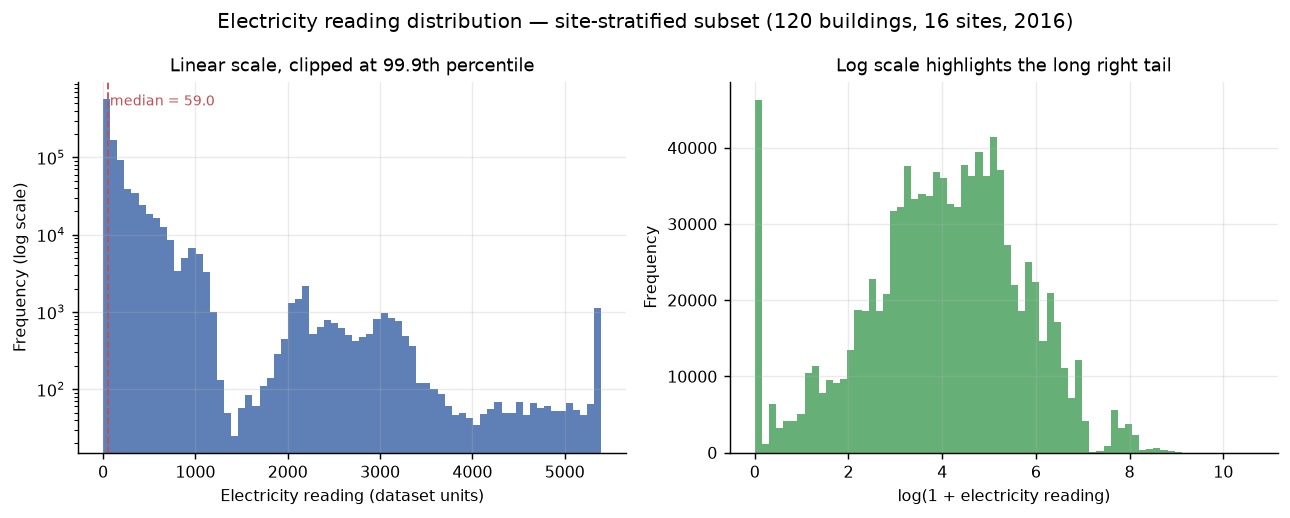
\includegraphics[width=\linewidth]{../reports/figures/reading_distribution.png}\\
\scriptsize Median 59.05 vs mean 188.78; p99 2,454; heavy right tail.
\end{block}

\begin{block}{Size is a strong, interpretable signal}
\centering
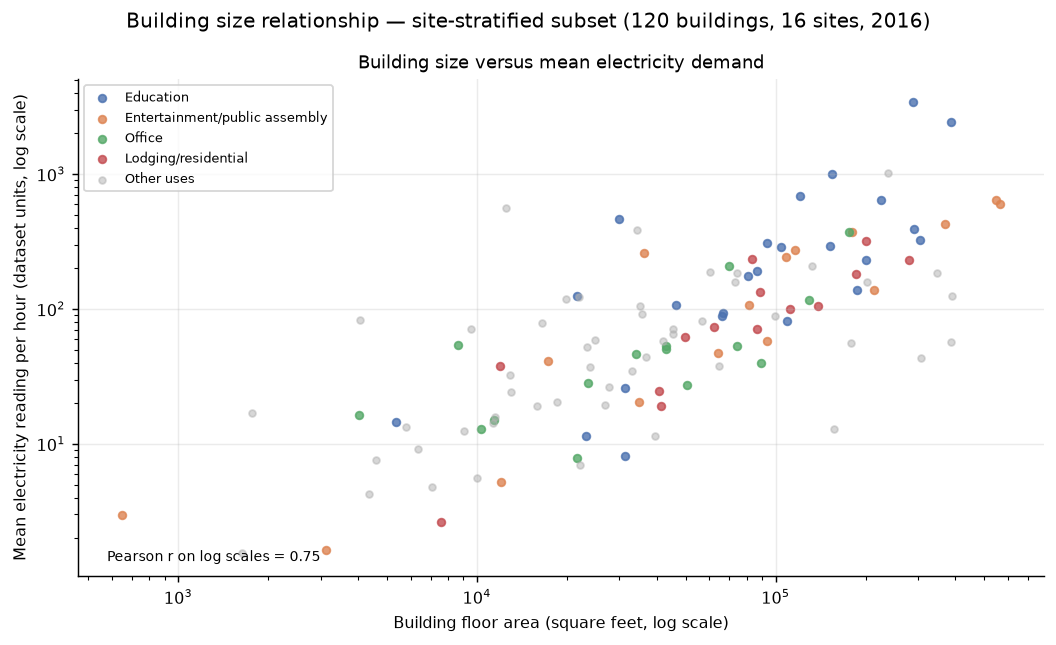
\includegraphics[width=\linewidth]{../reports/figures/building_size_relationship.png}\\
\scriptsize Log floor area vs log reading: $r=0.750$; useful for segmented benchmarking.
\end{block}
\end{column}

% ================= COLUMN 2 =================
\begin{column}{0.315\paperwidth}
\begin{block}{5. Methodology}
\small
\textbf{Pipeline:} raw CSVs $\rightarrow$ typed Parquet $\rightarrow$ electricity filter $\rightarrow$ metadata/weather joins $\rightarrow$ feature engineering $\rightarrow$ chronological split $\rightarrow$ pipelines $\rightarrow$ validation $\rightarrow$ test $\rightarrow$ error/generalization analysis $\rightarrow$ dashboard extracts.\\[0.1cm]
\textbf{Chronological split:} train Jan--Sep 2016; validation Oct--Nov; test Dec. No random shuffling across time.
\end{block}

\begin{block}{6. Models and selection}
\begin{center}
\begin{tabular}{p{0.39\linewidth}p{0.54\linewidth}}
\toprule
Model & Key configuration\\
\midrule
Linear Regression & One-hot; median impute; scale\\
Random Forest & 80 trees; depth 16; 250k sample\\
HistGradient\-Boosting & 200 iters; lr 0.08; 31 leaves\\
\bottomrule
\end{tabular}
\end{center}
\small Selection rule: \textbf{lowest validation RMSE}. Test evaluated once after selection. Seed 42. Metrics: MAE, RMSE, R$^2$, RMSLE.
\end{block}

\begin{block}{7. Results}
\begin{center}
\small
\begin{tabular}{lrrrr}
\toprule
Model & Test MAE & Test RMSE & Test R$^2$ & RMSLE\\
\midrule
Mean baseline & 209.57 & 406.05 & $-0.001$ & 1.920\\
Linear Regression & 61.39 & 154.51 & 0.855 & 0.942\\
Random Forest & \textbf{32.05} & 78.90 & 0.962 & \textbf{0.448}\\
HistGradient\-Boosting & 33.20 & \textbf{69.78} & \textbf{0.970} & 0.591\\
\bottomrule
\end{tabular}
\end{center}
\small
\textbf{Selected:} HistGradientBoosting, by validation RMSE (165.74 vs 166.92). Random Forest has lower MAE and RMSLE; the trade-off is reported. HGB fit about 4.3$\times$ faster.
\end{block}

\begin{block}{Diagnostics: errors concentrate at high demand}
\centering
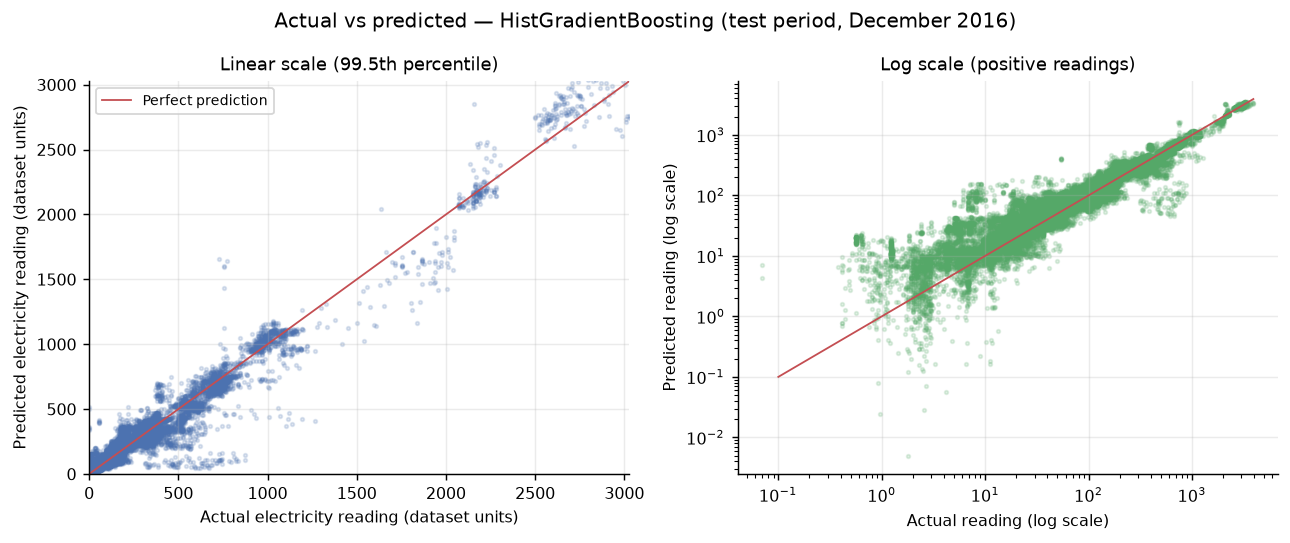
\includegraphics[width=\linewidth]{../reports/figures/actual_vs_predicted.png}\\
\scriptsize Test actual vs predicted; the 45$^\circ$ line is a perfect forecast. High-demand points are harder.
\end{block}

\begin{block}{What drives the model}
\centering
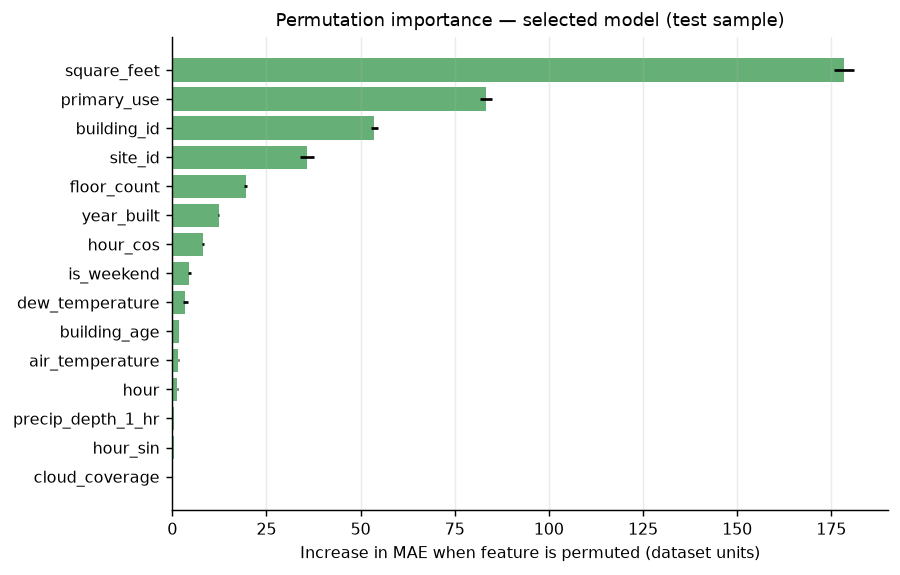
\includegraphics[width=\linewidth]{../reports/figures/feature_importance.png}\\
\scriptsize Building identity dominates; weather and hour add useful signal.
\end{block}

\begin{block}{Occupancy creates a weekday/midday cycle}
\centering
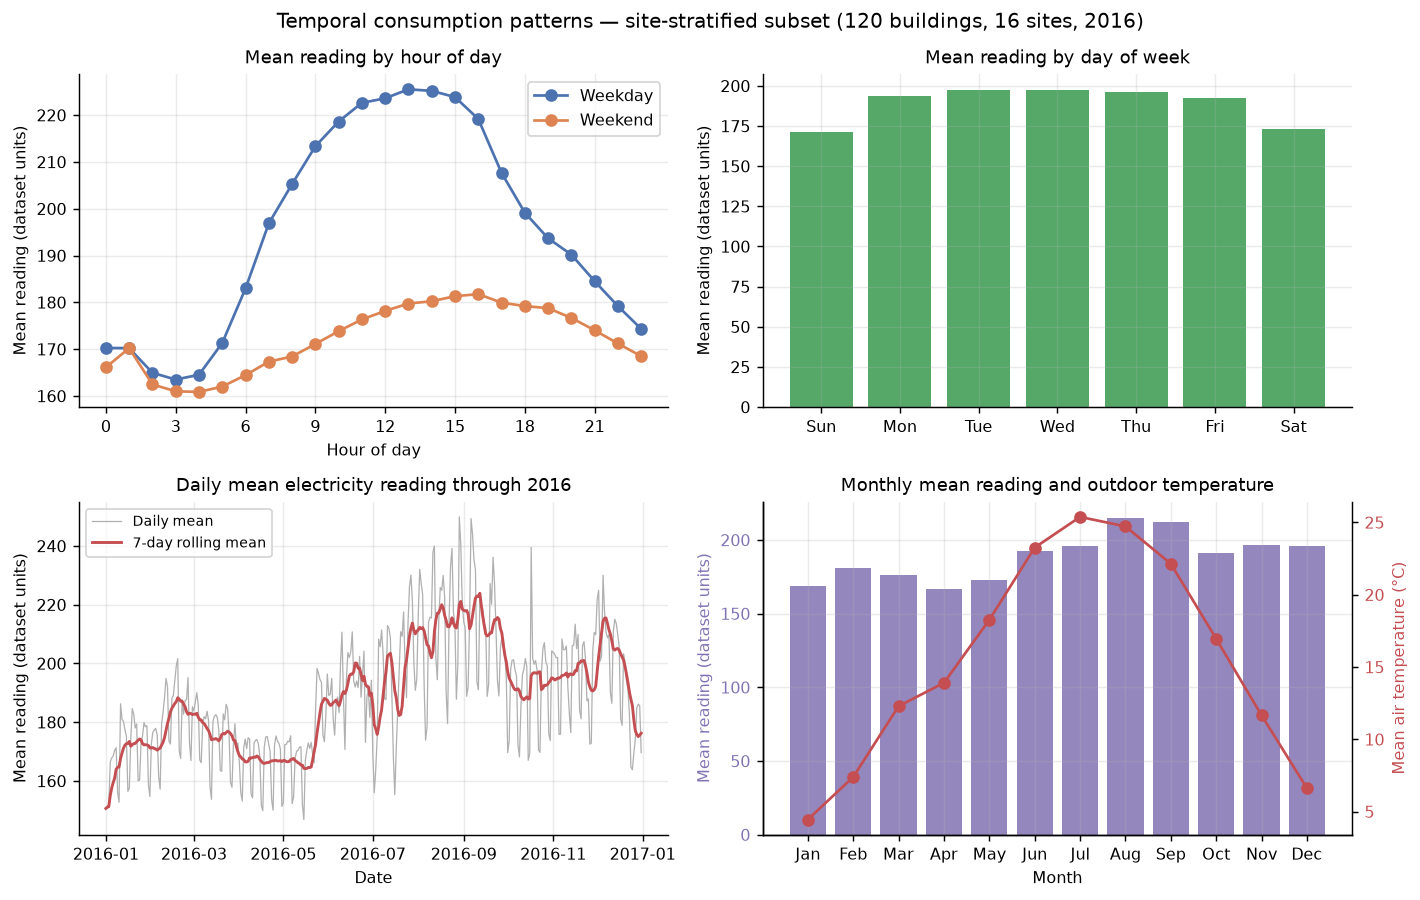
\includegraphics[width=\linewidth]{../reports/figures/temporal_patterns.png}\\
\scriptsize Weekday mean 195.44 vs weekend 172.24; peak 13:00, trough 03:00.
\end{block}
\end{column}

% ================= COLUMN 3 =================
\begin{column}{0.315\paperwidth}
\begin{block}{8. Critical finding: unseen buildings}
\begin{center}
\small
\begin{tabular}{lrrrr}
\toprule
Group & MAE & RMSE & R$^2$ & RMSLE\\
\midrule
Seen buildings, test & 33.86 & 74.15 & 0.971 & 0.595\\
Unseen buildings, test & 150.51 & 321.33 & $\mathbf{-0.555}$ & 1.525\\
\bottomrule
\end{tabular}
\end{center}
\begin{tcolorbox}[colback=paleorange,colframe=orange,boxrule=1.2pt,arc=2pt,left=4pt,right=4pt,top=3pt,bottom=3pt]
\small
\textbf{High seen-building R$^2$ is building-specific interpolation, not a universal physical model.} The model relies on \emph{building\_id}. Unseen predictions are biased high (242.49 vs 176.99). Do not deploy to new buildings without calibration or richer descriptors.
\end{tcolorbox}
\end{block}

\begin{block}{Unseen building holdout}
\centering
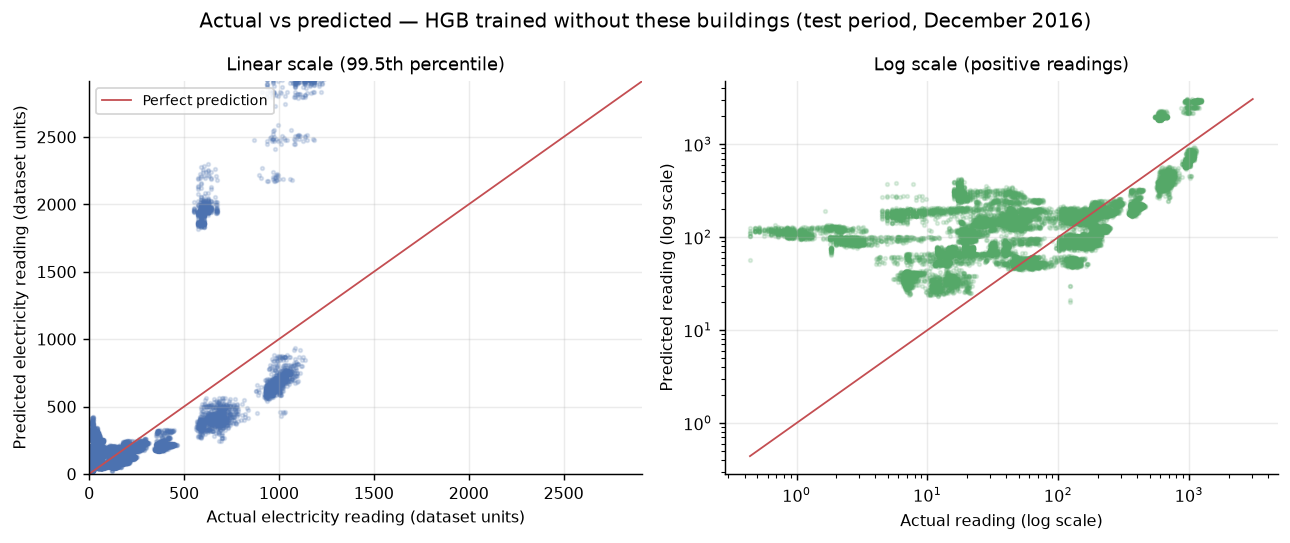
\includegraphics[width=\linewidth]{../reports/figures/unseen_buildings_actual_vs_predicted.png}\\
\scriptsize Building holdout: predictions compress toward the mean, giving negative $R^2$.
\end{block}

\begin{block}{9. Unseen-case demonstrations}
\begin{center}
\small
\begin{tabular}{lrrr}
\toprule
Case & Actual & Predicted & Error\\
\midrule
Building 1088, 19 Dec 15:00 & 3,427.60 & 3,417.33 & 0.30\%\\
Building 386, 9 Dec 06:00 & 41.16 & 41.16036 & 0.0009\%\\
\bottomrule
\end{tabular}
\end{center}
\small The near-exact second case is not proof of generalization; trees can match a leaf closely. The building-holdout experiment is the real test.
\end{block}

\begin{block}{10. Five engineering insights}
\small
\begin{itemize}
\item \textbf{Demand is right-skewed and building-dominated.} Median 59.05 vs mean 188.78; floor-area log correlation 0.750. Benchmark within use/size groups.
\item \textbf{Occupancy schedules create a weekday/midday cycle.} Weekday 195.44 vs weekend 172.24; peak 13:00, trough 03:00. Target setback studies.
\item \textbf{Temperature response is site-specific.} Pooled $r=-0.074$, but site $r$ ranges $-0.134$ to $+0.406$. Use degree hours or site interactions.
\item \textbf{Primary use and site dominate.} Median reading 3.75--157.20 by use; site means 10.24--1,156.11. Segment reporting.
\item \textbf{Seen-building accuracy does not transfer.} $R^2$ 0.970 seen vs $-0.555$ unseen. Recalibrate before new-building use.
\end{itemize}
\end{block}

\begin{block}{Temperature response is site-specific}
\centering
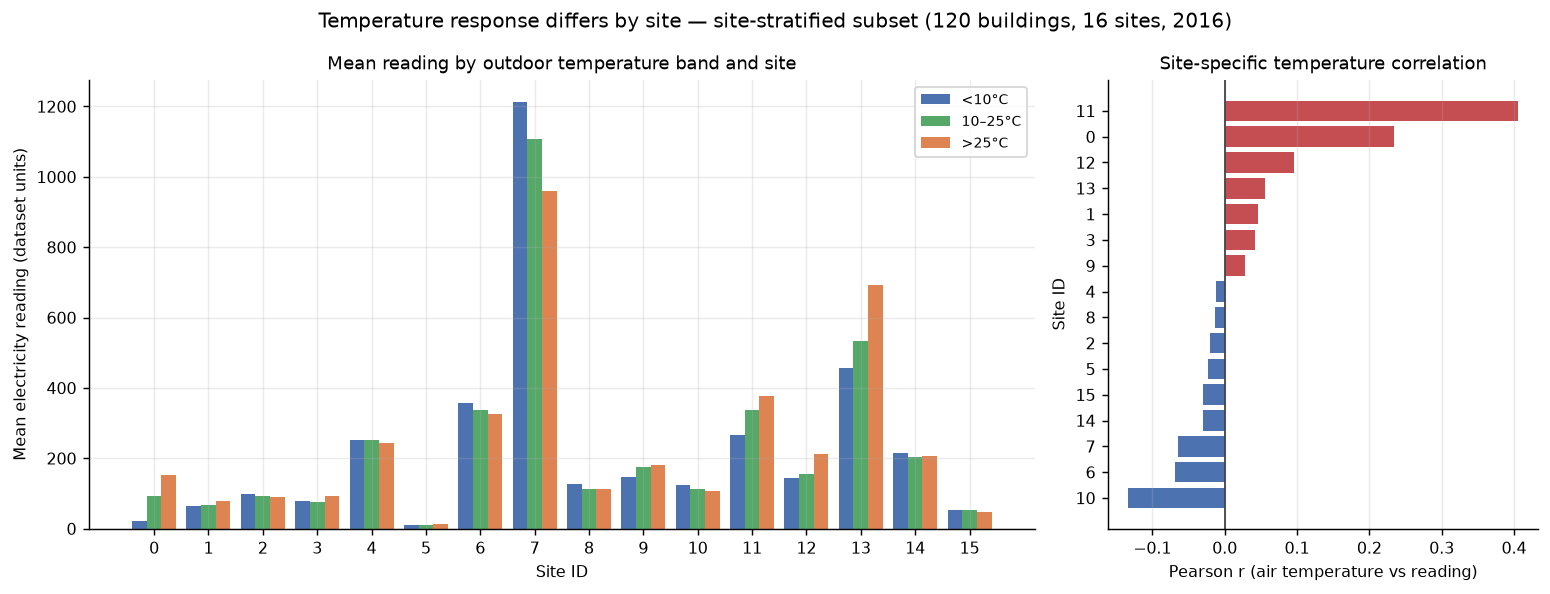
\includegraphics[width=\linewidth]{../reports/figures/temperature_response_by_site.png}\\
\scriptsize Pooled correlation masks opposite heating and cooling regimes.
\end{block}

\begin{block}{11. Dashboard and reproducibility}
\small
\textbf{Tableau-ready extracts:} 1,030,967 electricity rows; 349,232 prediction rows; 144 MB total. Spec covers overview, demand, weather, model performance, and data quality.\\[0.1cm]
\textbf{Streamlit supplement:} four pages (Overview, Weather \& Buildings, Model Performance, Predict), smoke-tested with no exceptions.\\
\textbf{Tableau workbook is pending user authoring.} Notebook, tests, README, and technical report are in the repository.
\end{block}

\begin{block}{12. Reproducibility and status}
\small
\begin{itemize}
\item 22 automated tests pass; the 23-cell notebook (13 code cells) executed with saved outputs.
\item Commands: \texttt{python -m src.data\_loading}; \texttt{python -m src.train\_models}; \texttt{streamlit run dashboard/streamlit\_app.py}.
\item Full-data Colab path is documented; local subset results are the only metrics reported.
\item Dataset approval and the Tableau workbook remain pending.
\end{itemize}
\end{block}
\end{column}
\end{columns}

\vspace{0.25cm}
\begin{tcolorbox}[colback=lightgrey,colframe=teal,boxrule=1pt,arc=2pt,left=5pt,right=5pt,top=3pt,bottom=3pt]
\small
\begin{columns}[t]
\begin{column}{0.24\linewidth}
\textbf{Conclusion.} The model is a useful \textbf{seen-building monitoring and interpolation tool}, not a validated new-building predictor. Results are from a 120-building subset, one year, a winter test month, site-level weather, and substantially missing metadata.
\end{column}
\begin{column}{0.24\linewidth}
\textbf{Recommendations.} Add past-only history features; add degree hours and site interactions; model zero/non-zero separately; calibrate residuals by building and load band; validate on a future year and a building holdout; build and verify the Tableau workbook.
\end{column}
\begin{column}{0.24\linewidth}
\textbf{Limitations.} One year; one winter test month; site-level weather; missing metadata; dataset units not independently verified; zero inflation; no causal claims; no full-data metrics; no Tableau workbook yet.
\end{column}
\begin{column}{0.24\linewidth}
\textbf{References.} ASHRAE (2019), \emph{Great Energy Predictor III}, Kaggle. Miller et al. (2020), \emph{Science and Technology for the Built Environment}, 26(10), 1427--1447. Amasyali \& El-Gohary (2018), \emph{Renewable and Sustainable Energy Reviews}, 81, 1192--1205.
\end{column}
\end{columns}
\vspace{0.08cm}
\scriptsize Status: local subset complete; Tableau workbook pending; full-data run pending; dataset approval pending. Code and report: README.md, reports/technical\_report.md, reports/engineering\_insights.md.
\end{tcolorbox}
\end{frame}
\end{document}
